%%%%%%%%%%%%%%%%%%%%%%%%%%%%%% Recordatorios

% El levantamiento de la encuesta va de 01/11/2018 a 23/11/2018, pero oficialmente en la base de datos se tienen registros de 2020 y 2013 y 4 registros en el dia 0

%%%%%%%%%%%%%%%%%%%%%%%%%%%%%% Paquetes

\documentclass{article}
\usepackage[utf8]{inputenc}
\usepackage[spanish]{babel}
\usepackage[affil-it]{authblk}
\usepackage{hyperref}
\hypersetup{
    colorlinks=true,
    linkcolor=blue,
    filecolor=magenta,      
    urlcolor=cyan,
    pdftitle={Overleaf Example},
    pdfpagemode=FullScreen,
    }
\usepackage[usenames]{color}

\usepackage{graphicx}

\usepackage{graphics} % Para desplegar imágenes

\usepackage{subfig}
\usepackage[verbose]{placeins}

\usepackage[left = 50, right = 65, top = 40, bottom = 40]{geometry}
%%%%%%%%%%%%%%%%%%%%%%%%%%%%%% Preambulo
\setlength{\parindent}{0cm}
\title{Proyecto Final Muestreo: Análisis descriptivo sobre las preferencias de los contratantes de actuarios recién egresados en el año 2018. }
\author{David Montaño Castro}
\affil{Facultad de Ciencias, Universidad Nacional Autónoma de México.}
\date{\today}

\makeatletter
\def\@maketitle{%
  \newpage
  \null
  \vskip 2em%
  \begin{center}%
  \let \footnote \thanks
    {\Large\bfseries \@title \par}%
    \vskip 1.5em%
    {\normalsize
      \lineskip .5em%
      \begin{tabular}[t]{c}%
        \@author
      \end{tabular}\par}%
    \vskip 1em%
    {\normalsize \@date}%
  \end{center}%
  \par
  \vskip 1.5em}
\makeatother

%%%%%%%%%%%%%%%%%%%%%%%%%%%%%% Configuraciones del Documento
 
\begin{document}
\maketitle
\begin{abstract}
    El presente análisis descriptivo tiene por objetivo el entender cómo y cuáles eran las preferencia y habilidades más demandadas por los contratantes de actuarios recién egresados al momento de que estos últimos iniciaran su vida laboral. A lo largo del presente documento se pone en evidencia el gran campo laboral en el que los actuarios pueden desarrollarse; así mismo, los datos revelan la falta de preparación técnica y práctica por parte de los graduados al momento de enfrentarse a su primer experiencia laboral.  
    
    \textbf{Palabras Clave:} actuaría, actuario , egresados, UNAM .
\end{abstract}
\tableofcontents
\newpage

%%%%%%%%%%%%%%%%%%%%%%%%%%%%%% Documento



\section{INTRODUCCIÓN}

\subsection{Ser actuario en México}

El \href{http://oferta.unam.mx/actuaria.html}{sitio oficial de la UNAM} define a un actuario como:

\begin{center}
    "Profesionistas que estudian, plantean, formulan y aplican modelos de contenido matemático con el fin de proveer información para la planeación, previsión y toma de decisiones, y para resolver problemas económicos y sociales que involucran riesgos. Intervienen en prácticamente todos los campos del quehacer humano interactuando con los profesionales que ahí se desempeñen."
\end{center}
    
En primera instancia podría parecer un párrafo poco informativo, pues más concretamente "¿Entonces qué sabe hacer un actuario?":

\begin{center}
    "Llevan a cabo una labor sumamente diversa y relacionada principalmente con: seguros y planes de beneficio, demografía, finanzas, computación, administración, estadística, investigación de operaciones, economía, docencia e investigación."
\end{center}

Queda claro que la profesión de un actuario va más allá de lo matemático. A diferencia de otros campos de las ciencias exactas, la actuaría requiere al profesionista de diversas habilidades sociales y culturales para poder lograr un enlace armonioso entre lo matemático y social. Esta profesión en México es relativamente nueva y por lo tanto, brinda a los estudiantes universitarios un sentido de tranquilidad a la hora de embarcarse en la vida laboral. \\

No obstante, lo novedoso no siempre es sinónimo de perfección. A pesar de que la tasa de empleados recién egresados de la UNAM es de $81\%$ \footnote{Periodo del año 2021.}, no se tiene con claridad el panorama de lo que los planes de estudio en México plantean ni qué tan útiles resultan laboralmente hablando. Esto se traduce en posibles deficiencias y carencias por parte de los egresados al desempeñar sus primeros trabajos, generando desconfianza en las empresas.
 
\section{OBJETIVO}

Llevar a cabo un estudio descriptivo sobre las preferencias de los contratantes de actuarios recién egresados en distintas áreas del conocimiento para poder esclarecer cuáles son las áreas de oportunidad en las cuales los actuarios deban focalizar mayormente su atención en aras de tener los conocimientos y elementos necesarios para ser competentes en el mercado laboral.  

\section{METODOLOGÍA}

\begin{enumerate}
    \item Descargar el conjunto de datos \textit{BASE DE CONTRATANTES 2018 V2.csv}, diseñada y proveída por el profesor Francisco Villareal. 
    
    \item Analizar, depurar y seleccionar los atributos del conjunto que proporcionan información relevante y baste para el estudio.
    
    \item Proporcionar un análisis descriptivo univariado por medio de gráficas y frecuencias sencillas de comprender. Esto con el fin de entender cómo está diseñada y distribuida la información.
    
    \item Realizar un análisis descriptivo 'bi' y trivariado que permita estratificar de una mejor manera las aptitudes y habilidades necesarias que los egresados deberían de tener dependiendo del área a la cual les gustaría dedicarse. De igual manera se integran representaciones visuales y tabulares para una interpretación más dócil.
    
    \item Llevar a cabo un análisis de recuperación en textos para analizar opiniones y comentarios de los entrevistados. 
    
\end{enumerate}

\section{PROCEDIMIENTO}

\subsection{Herramientas computacionales}

Todos los procedimientos estadísticos se realizaron utilizando el lenguaje de programación \textit{Python} (Versión 3.8.3) junto con \textit{Excel} para representaciones visuales de mayor conveniencia que no podían ser diseñadas en \textit{Python} ($100\%$ stackedbars). Para \textit{Python}, se requieren las librerías \textit{Pandas} (manejo y depuración del conjunto de datos), \textit{Matplotlib} y \textit{Seaborn} (representaciones visuales), \textit{Numpy} (estadísticos básicos), así como \textit{Scipy, FuzzyWuzzy y WordClouds.}. \\


\subsection{Estructura del conjunto de datos}

El conjunto de datos tiene formato \textit{csv}. Consta de 282 registros únicos y 108 columnas con tipo de datos \textit{float64} (5), \textit{int64} (28) y \textit{object} (75). \\

En ningún momento se imputaron datos; en su lugar, los valores faltante fueron retirados del estudio. El conjunto contenía columnas (22) con más de $95\%$ de datos faltantes, por lo cual desde un inicio fueron retiradas verificando que la ausencia de datos no significaran la ausencia de algún atributo que pudiera aportar información importante.  \\

El levantamiento de la encuesta tuvo lugar del día 01/11/2018 al 23/11/2018, pero oficialmente en la base de datos se tienen registros de 2020 (1) y 2013 (1) y 4 registros en el dia 0/11/2018, fechas las cuales se atribuyen a errores humanos de captura. \\

En particular, todos los atributos textuales contienen errores gramaticáles, ortográficos y de sintaxis. Aquellas columnas cuya función es una mejor categorización y estratificación de la muestra, fallan en su acometido debido a la falta de estructura; es decir, cada entrevistado podía responder libremente y sin ninguna condición de formato, lo cual causa que encontremos registros tales como 'Jefa' y 'Jefe', 'actuaría' y 'actuario'\footnote{Esto es, existen sinónimos en una misma clasificación. Una tarea muy difícil es clasificar textos de manera no supervisada, el cual es el caso en esta encuesta.}, etc. Por lo tanto, tuvieron que emplearse algunas técnicas básicas de recuperación de información en textos para poder sacar valor de estos atributos. 

\subsection{Análisis univariado}

El análisis presentado en esta sección es una breve mirada a la distribución de los datos. El principal objetivo es describir tanto como se pueda de cada atributo para poder formular preguntas más completas que aporten valor y conocimiento a los lectores. Mayoritariamente se muestran gráficas a modo de resumen y se limitan las tabulaciones en pos de una lectura rápida. En conjunto con las representaciones visuales se sustenta con una breve descripción de la interpretabilidad inherente a cada elemento. \\

Es importante destacar que \textbf{aquellos atributos analizados textualmente fueron tratados por medio de la Distancia de Levenshtein}; no obstante, esta técnica rápidamente se vio afectada en tiempo y tamaño de muestra, obligándome a filtrar y limpiar los textos de manera manual y con ayuda de \textbf{Expresiones Regulares}. Dado que este análisis es puramente univariado, aquellos registros que no eran sencillamente generalizables simplemente se mandaron a una clasificación del tipo 'otros'. En adición, se emplearon herramientas como \textbf{WordClouds}\footnote{Del inglés, Nube de Palabras.} ya que resumen de manera inmediata las palabras más frecuentes en un conjunto de textos de manera intuitiva y muy visual.

Para cerrar, se trabajaron con aquellos datos que tuvieran información disponible. Por lo tanto, hay que tener en consideración que los porcentajes y el número de personas no será siempre el mismo a lo largo de cada descripción. 

\subsection{Análisis Bi/Tri-variado}

El análisis presentado en esta sección ya integra tanto de manera visual como tabular dos o tres atributos. El objetivo principal es \textbf{estratificar la muestra por Actividad Principal de la Institución en donde los entrevistados trabajan.} 

\begin{itemize}
    \item Los datos numéricos fueron tratados como variables ordinales en una escala Likert de 5 elementos (en su mayoría). Este hecho no permitirá el cálculo de frecuencias como la media o la mediana, más bien la moda. 
    
    \item La columna 'ACTP' fue asignada como la variable estratificadora y se divide en 8 clasificaciones\footnote{Las expresiones regulares para filtrar la información pueden verse en el script de Python. }:
    
    \begin{enumerate}
        \item ASEGURADORA;
        
        \item CONSULTORÍA;
        
        \item BANCO;
        
        \item PRODUCTOS / SERVICIOS FINANCIEROS;
        
        \item ANÁLISIS;
        
        \item FARMACÉUTICA;
        
        \item ALIMENTOS;
        
        \item RH;
        
        \item DOCENCIA
    \end{enumerate}
    
\end{itemize}

Dichas clasificaciones fueron meramente subjetivas. Se miró simultáneamente al nombre de la empresa y a la actividad \textit{per se} para tener una mejor idea de aquellos registros que eran tan generales como para poder asignarles una clasificación sencillamente. En general, \textbf{se buscaban palabras homónimas para luego agruparse de manera manual.} No siempre fue posible encontrar una clasificación y por lo tanto, durante este análisis se contará con un \textbf{máximo de 234 registros} por cada sección. \footnote{Es decir, 46 registros no pudieron ser asignados a una clasificación por ambigüedad. Puede ser menor la cantidad de registros dependiendo de la disponibilidad de datos.}
    
\subsection{Análisis no paramétrico}

En ésta última sección se efectúa un análisis de diferencia de medias \textit{Kruskal-Wallis}. Se dan las razonas por las cuales no es útil (ni siquiera válido) implementar este tipo de análisis con la información recabada y restante de la encuesta. 
    
\newpage

\section{RESULTADOS}

\subsection{Univariado}

\subsubsection{Número de empresas únicas en el estudio}

Hay un total de \textbf{188 empresas únicas} en el estudio, de las cuales las siguientes 5 tuvieron mayor número de registros:

\begin{enumerate}
    \item CNSF;
    
    \item BBVA BANCOMER;
    
    \item BANORTE;
    
    \item METLIFE;
    
    \item GRUPO MEXICANO DE SEGUROS
\end{enumerate}

\subsubsection{Cargo de los entrevistados}

\begin{center}
    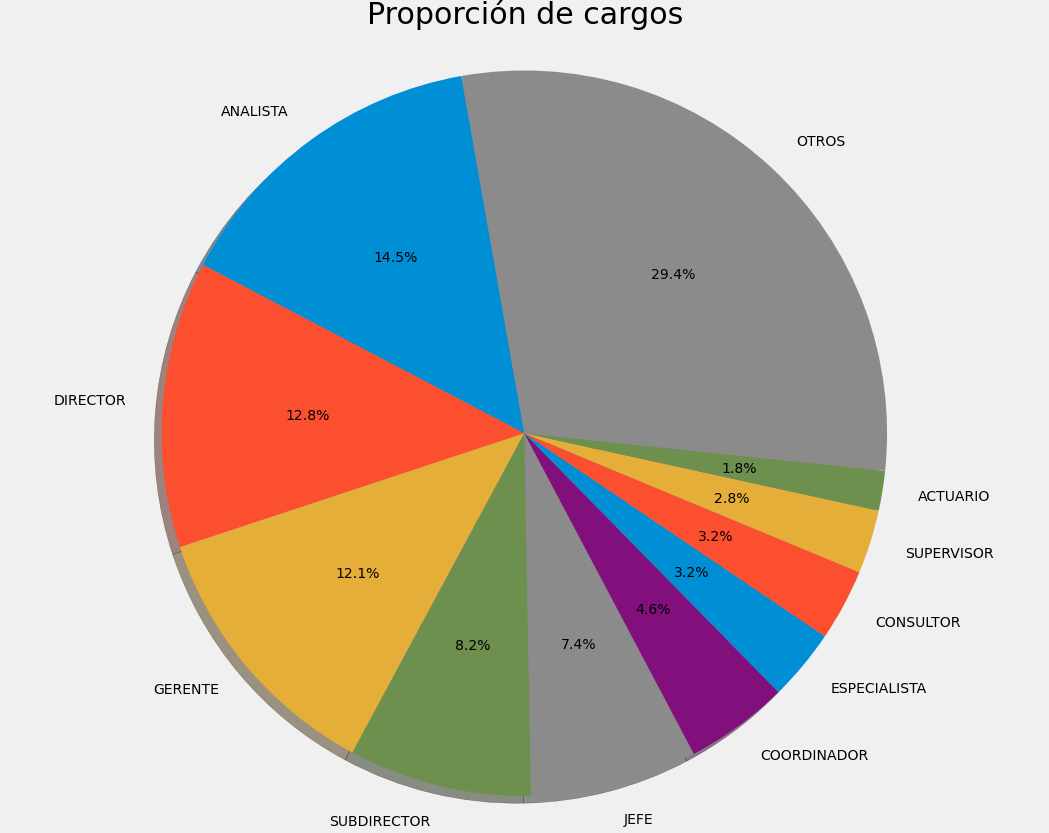
\includegraphics[scale = 0.3]{1cargos}
\end{center}

Poco más del $70\%$ de respuestas provienen de personas con experiencia, pues estos cargos requieren de conocer bien el sector en el que se desarrollan. La lista está liderada por Analistas ($14.5\%$), Directores ($12.8\%$) y Gerentes ($12.1\%$). Las demás categorías son incluso más elevadas que un Gerente, reafirmando la confianza con la que podemos confiar en sus opiniones plasmadas en esta encuesta. 

\subsubsection{Sector}

En la encuesta se tiene la presencia de $68\%$ de empresas privadas y $32\%$ públicas.

\subsubsection{Actividad Principal de la Institución}

\begin{center}
    
\includegraphics[scale = 0.3]{2ACTP.png}
\end{center}

Los actividades principales más representativas de las instituciones en donde los entrevistados se desenvuelven son, por supuesto, \textbf{Aseguradoras, Financieras, Bancos y Consultarías}. Algunas otras actividades resaltables son la investigación de mercado, la creación de modelos, la supervisión de procesos, etc. Esto confirma la dicha de que los actuarios tienen presencia en muchas áreas del conocimiento por la diversificación tan exhaustiva de cursos que se toman a lo largo de la carrera; nuevamente, se aclara el panorama más esperanzador: seguros. 


\subsubsection{Funciones Principales}

\begin{center}
    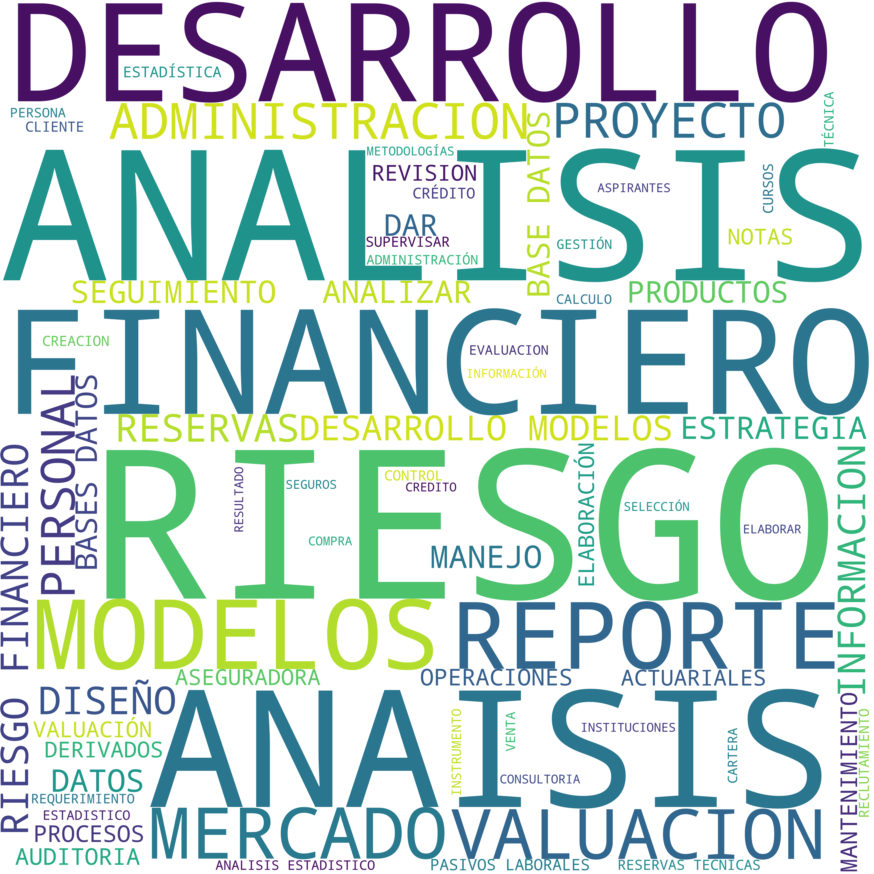
\includegraphics[scale = 0.3]{3FUN.png}
\end{center}

Entre las funciones principales que más destacan en el conjunto de datos están: \textbf{Análisis, Riesgos, Reportes, Valuación, Modelos, Diseño, Creación de Estrategias, Administración, etc}. Las tareas anteriormente descritas son el pan de cada día de un estudiante de actuaría, en particular a partir de los últimos semestres cuando empezamos a aplicar todos los conocimientos teóricos vistos en clase. 

\subsubsection{Carreras Afines}

\begin{center}
    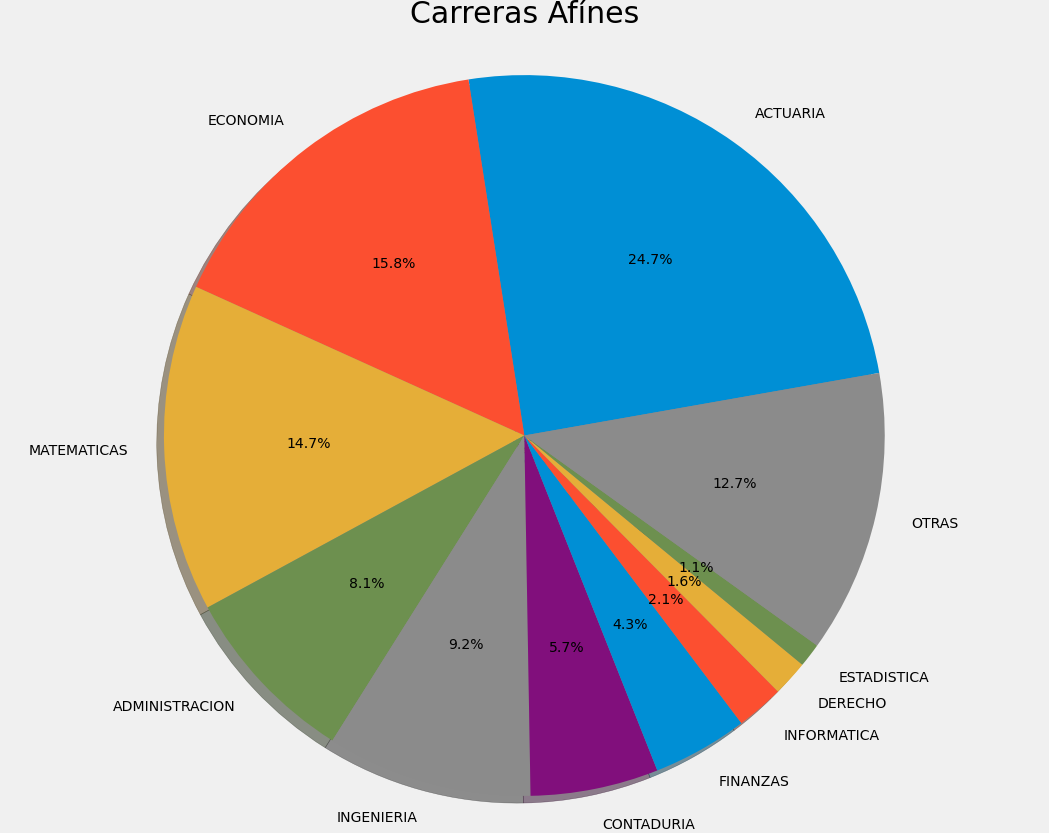
\includegraphics[scale = 0.3]{4CA.png}
\end{center}

Por supuesto, la encuesta está liderada por \textbf{Actuaría} como la carrera más afín en el ambiente laboral de los encuestados. Carreras como \textbf{Economía, Matemáticas, Administración, Ingeniería y Contaduría} encabezan los puestos subsecuentes, respectivamente. Esto propone una debilidad en nuestra preparación, pues el hecho de que el actuario tenga que desenvolverse en un ambiente más 'social' limita muchas veces su capacidad para explicar fundamentos y justificaciones a personas que no manejan lenguaje matemático (técnico). De igual manera, esto es una invitación a que dejemos de menospreciar a las carreras de área 3 (típico de área 1). Al final del día, trabajaremos mano a mano por un mismo objetivo. 


\subsubsection{Medios de contratación}

\begin{center}
    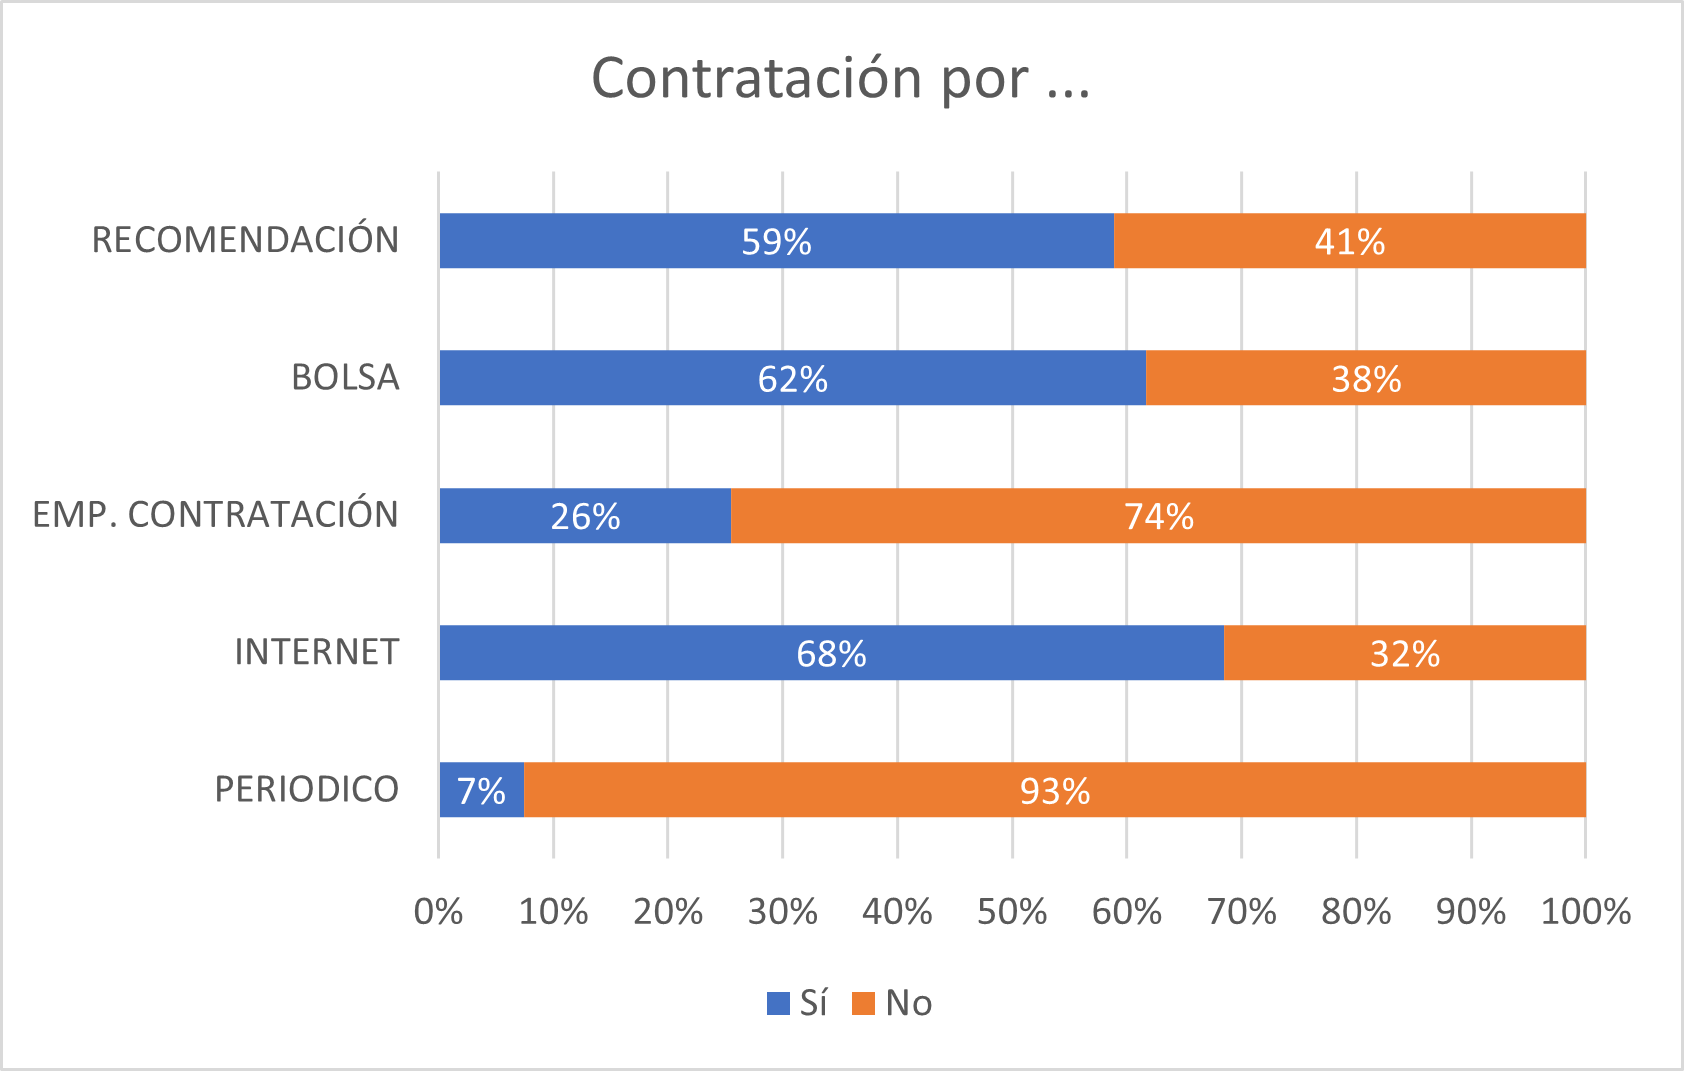
\includegraphics[scale = 1]{5MC.png}
\end{center}

El medio por excelencia para buscar trabajo desde hace ya algunos años sigue siendo \textbf{Internet}. Hay que remarcar la importancia de tener un circulo social extenso, pues las \textbf{recomendaciones} representan un porcentaje importante a la hora de buscar trabajo. Definitivamente la contratación por \textbf{Periódico} ha quedado en el pasado (al menos para actuaría).

\subsubsection{Requisitos Generales de Ingreso}

La \textbf{Edad} es, al menos para el $87\%$ de las personas encuestadas, irrelevante a la hora de contratar a un recién egresado de la carrera. \\

En cuestión de la contratación por \textbf{Género}, es técnicamente imposible ($1\%$) que exista una preferencia de género. En caso de que existiera, la encuesta sugiere que siempre es preferible una persona del género \textbf{femenino}. \\

Sobre la disposición de \textbf{Viajar}, el $66\%$ de los encuestados respondió que sí se requiere que el aspirante pueda efectuar viajes relacionados al trabajo. 

\subsubsection{Preparación Académica para el primer puesto}

\begin{center}
    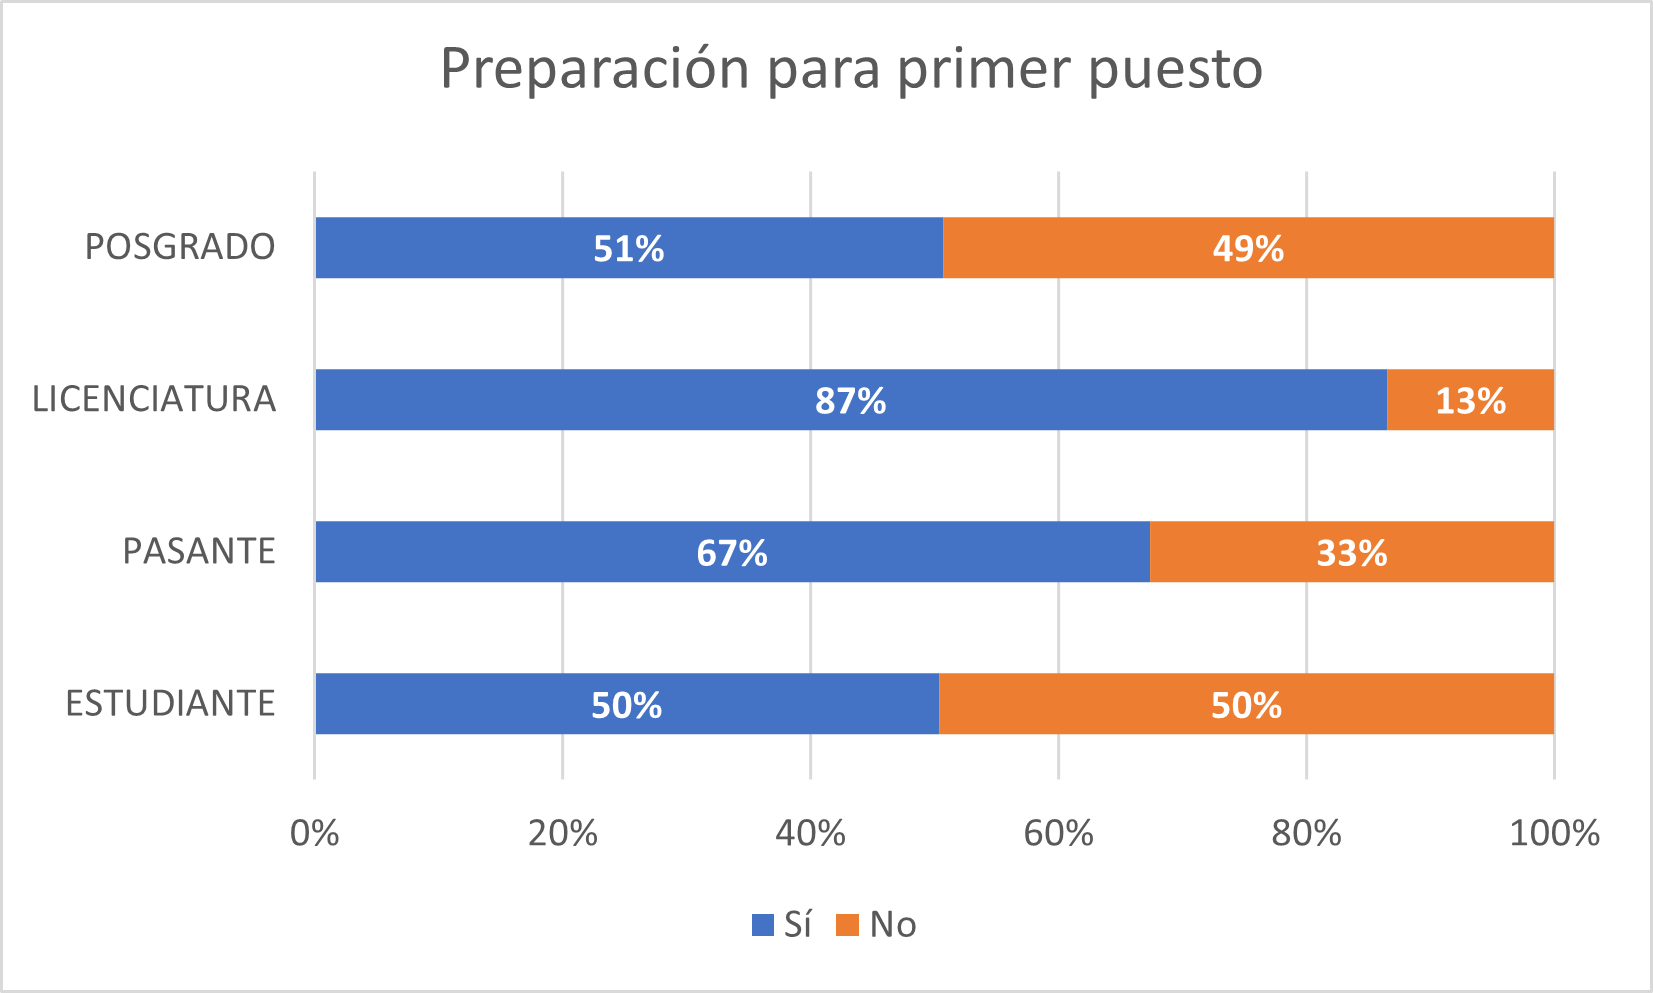
\includegraphics[scale = 0.9]{6PrimerTra.png}
\end{center}

Es más probable que un \textbf{recién egresado titulado} consiga un empleo a aquellos que siguen siendo \textbf{pasantes}. Existe el mito de que tener un posgrado a la hora de pedir un primer empleo (sin experiencia) puede llegar a ser contraproducente por la \textit{sobre calificación} para el puesto; la gráfica sugiere que esto podría ser cierto, pues \textbf{hay la misma probabilidad de ser contratado teniendo un posgrado a ser estudiante universitario}. \\

Con respecto al \textbf{Promedio mínimo} requerido por las empresas en donde los encuestados trabajan, solo el $30\%$ de los encuestados revelaron que éste es importante como requisito para poder aspirar a un puesto. De ésta porción, el rango del promedio mínimo es de \textbf{entre mínimo 8 y máximo 9}, siendo la primera cifra la más común ($78\%$).

\subsubsection{Dominio del idioma inglés}

\begin{center}
    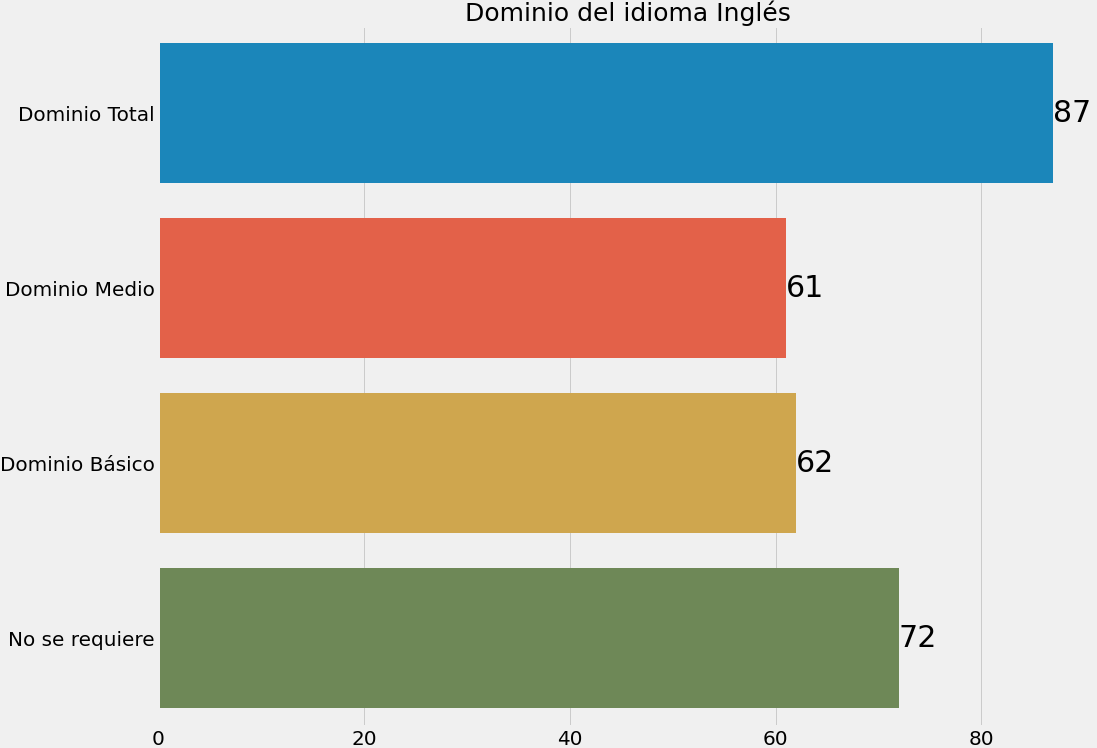
\includegraphics[scale = 0.3]{7Ingles.png}
\end{center}

El $30\%$ de las personas confesó que \textbf{es importante tener un dominio total del idioma inglés}; hecho que actualmente se mantiene e incluso con una tendencia al alza. Por otra parte, un $26\%$ declaró no necesitar saber inglés para conseguir un puesto dentro de la institución y $44\%$ restante considera un nivel medio como suficiente para llevar a cabo sus tareas.  

\subsubsection{Otros requisitos generales}

\begin{center}
    \includegraphics[scale = 0.3]{8ExpAños.png}
\end{center}

Contrario a lo que se cree, las empresas no consideran necesario ($67\%$) tener experiencia previa, es decir, que los estudiantes entran a algún programa de becariado durante sus estudios. Del $33\%$ que sí lo considera importante, en gran medida se desea que el aspirante \textbf{tenga de 1 a 3 años de experiencia, teniendo mayor frecuencia el año de experiencia}. 

\begin{figure}[h!]
\centering
\begin{minipage}{.5\textwidth}
  \centering
  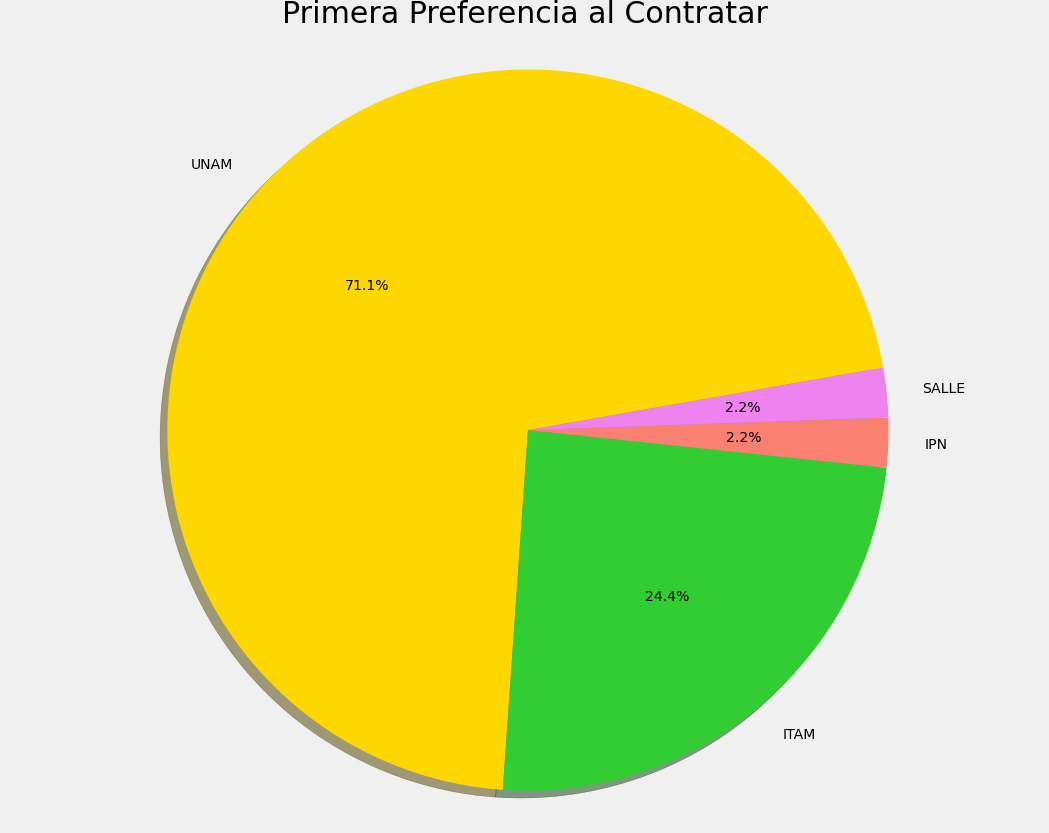
\includegraphics[scale = 0.26]{8primpref}
\end{minipage}%
\begin{minipage}{.5\textwidth}
  \centering
  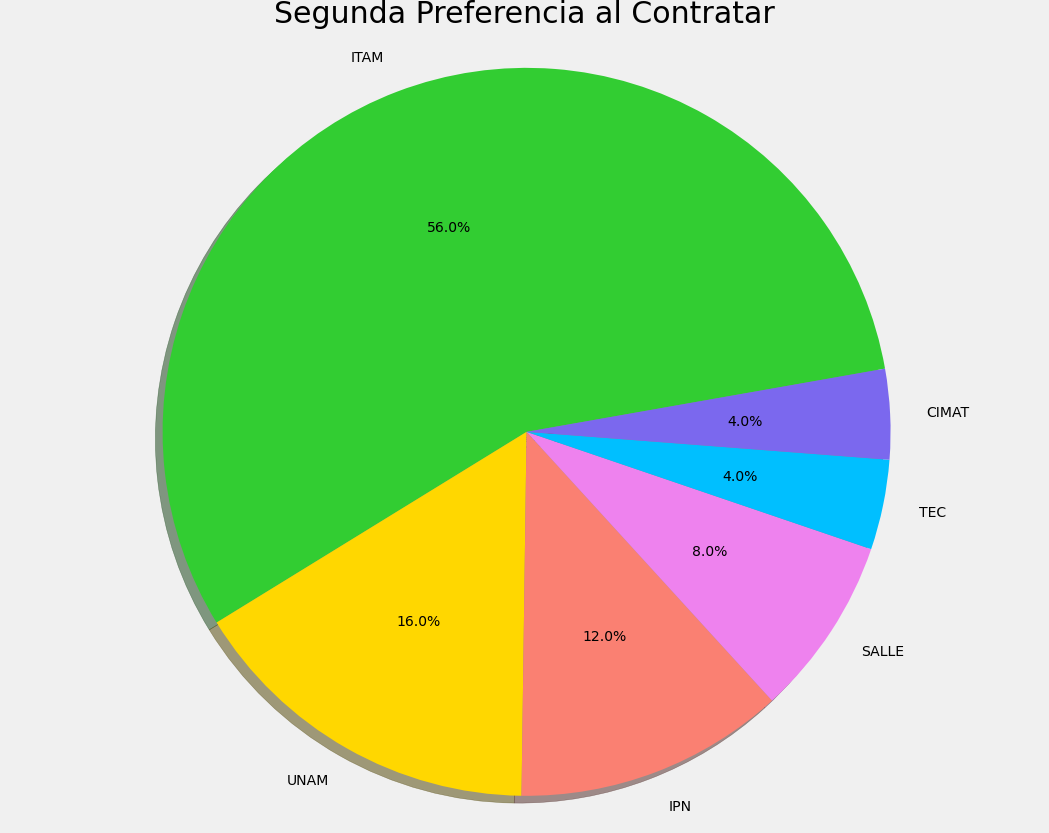
\includegraphics[scale = 0.26]{9segunpref}
\end{minipage}
\end{figure}

Además, pertinente a la \textbf{Preferencia por alguna universidad de origen}, el $82\%$ argumentó que no tienen una preferencia por alguna escuela en particular. Del resto, \textbf{como primera opción, la UNAM lidera con un $71\%$, siguiendo el ITAM con un $24\%$}. Como segunda preferencia, \textbf{el ITAM da la vuelta a la UNAM con un $56\%$ y $16\%$, respectivamente}. Diversas escuelas son consideradas como segunda opción: IPN, La Salle, el CIMAT y el TEC. En general, la UNAM resulta una escuela reconocida y de prestigio entre estas instituciones. 

\subsubsection{Personalidad de los aspirantes}

\begin{center}
    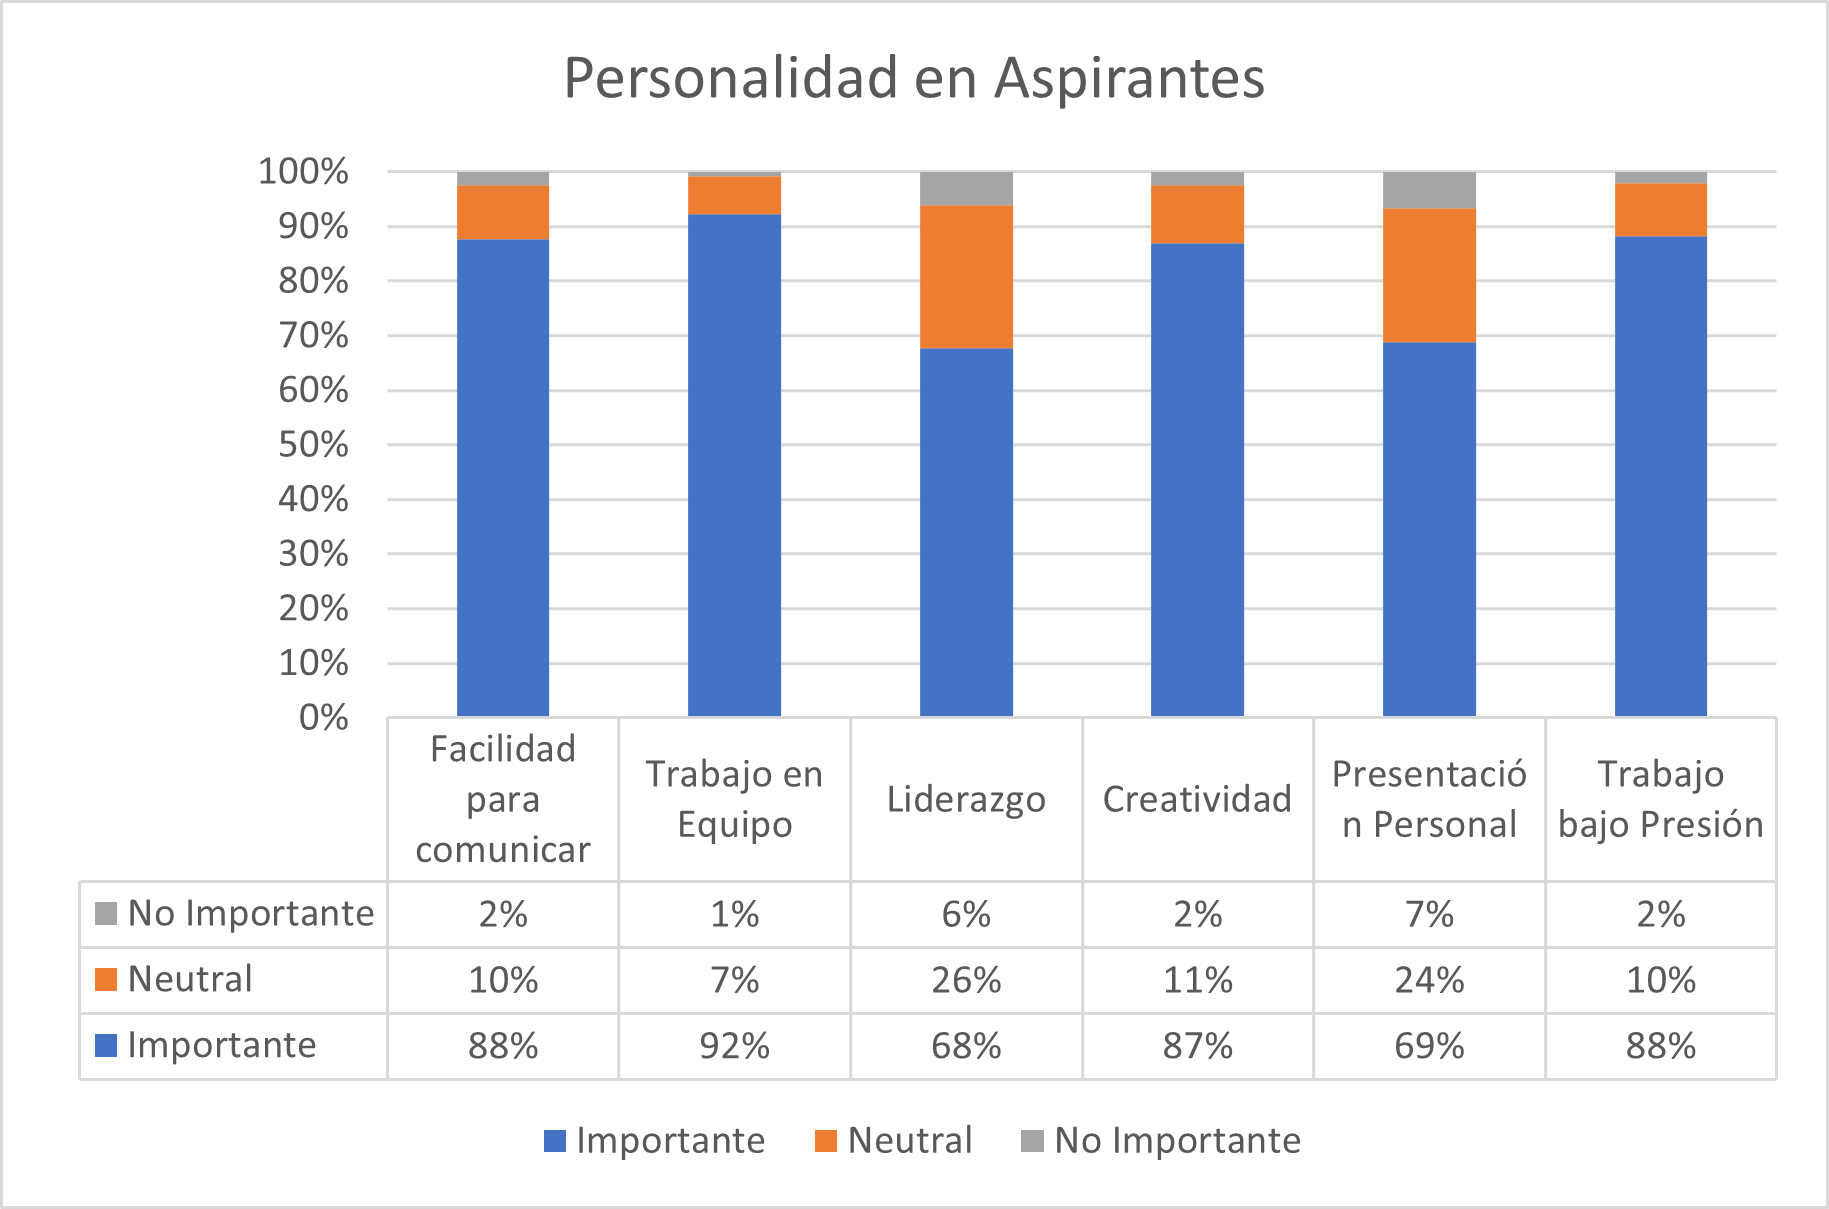
\includegraphics[scale = 0.9]{10personalidad.png}
\end{center}

El resultado es claro: sin importar la institución y a lo que se dediquen, \textbf{la Facilidad de palabra, el Trabajo en Equipo, el Liderazgo, la Creatividad, la Presentación Personal y el saber Trabajar Bajo Presión} son rasgos de personalidad muy apreciadas y requeridas por las empresas. En las escuelas debería de estimularse la necesidad de poner en práctica este tipo de habilidades blandas. 

\subsubsection{Conocimiento especializado por área}

\begin{center}
    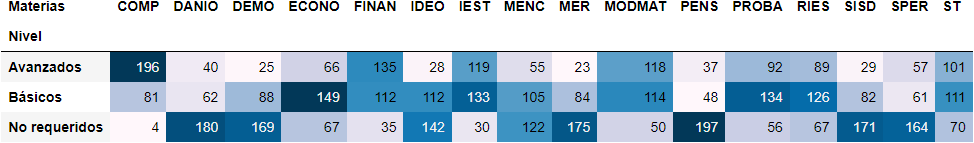
\includegraphics[scale = 0.7]{cono_cru_materias.png}
\end{center}

En general, pocas son las materias escolares que se requieren tener bien dominadas para acceder a un primer empleo; en estos casos, bien podría uno incursionarse con un nivel básico. Definitivamente \textbf{tener conocimientos avanzados de Computación} es crucial, así como de \textbf{Finanzas, Inferencia Estadística, Modelado Matemático y Series de Tiempo}. Estas materias corresponden a los últimos semestres de la carrera, pero para poder dominarlos a un nivel avanzado se requieren de todos los elementos matemáticos que se revisan durante los primeros semestres. 


\begin{center}
    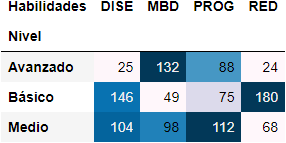
\includegraphics[scale = 0.85]{cono_cru_materias2.png}
\end{center}

Además, habilidades más especializadas como el \textbf{Manejo de Bases de Datos y la Programación} son de suma importancia para cualquier empresa que requiera egresados. En general \textbf{no se espera que los actuarios sepan de Redes ni de Desarrollo de Sistemas.}

\subsection{Bi/Tri-variado}

\subsubsection{¿Los años de experiencia que se solicita depende de la Actividad Principal de la empresa y del sector al que pertenece?}


\begin{center}
    \includegraphics[scale = 0.36]{graf_cru1_api_sec_expa_imagen.png}
\end{center}

En realidad son muy pocas las empresas que piden años de experiencia para dar una respuesta concreta. De manera muy (exageradamente) general, \textbf{el sector público en la actividad de Docencia pide más años en promedio de que las demás actividades. En el sector privado, la actividad Producción y Distribución de Alimentos es la que más años pide (1).}

\subsubsection{¿Qué carreras son más solicitadas por Actividad?}


\begin{figure}[h!]
\centering
\begin{minipage}{.5\textwidth}
  \centering
  \includegraphics[scale = 0.26]{graf_Primera_graf_cru2_api_ca.png}
\end{minipage}%
\begin{minipage}{.5\textwidth}
  \centering
  \includegraphics[scale = 0.26]{graf_Segunda_graf_cru2_api_ca.png}
\end{minipage}
\end{figure}

Actuaría domina en casi todas las áreas, exceptuando por Productos y Servicios Financieros, en la cuál Contaduría juega un papel importante. al igual que Informática. En la Actividad Farmacéutica tanto Ingeniería como Administración dominan la demanda. Es importante destacar que, en cuanto a las aseguradoras, las carreras que más se suelen contratar son Matemáticas y Economía, un comportamiento similar se visualiza en la Actividad Bancaria. Un panorama más desalentador es para los físicos, pues en ningún área parecen tener presencia importante. 



\subsubsection{¿Por qué medio me conviene aplicar para un trabajo dependiendo de la actividad a la que quiera especializarme?}

\begin{center}
    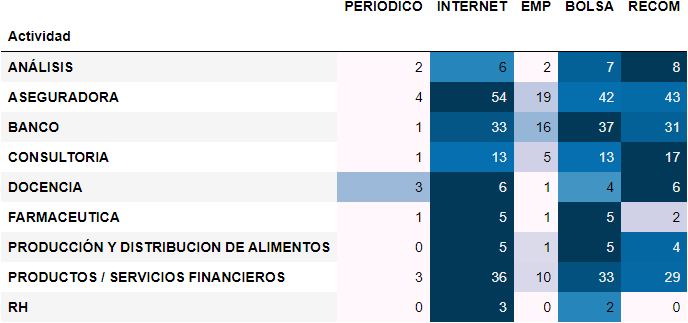
\includegraphics[scale = 0.8]{graf_api_contra.png}
\end{center}

No hay dudas: \textbf{el internet es la manera más efectiva para buscar un trabajo}. Su rapidez y sencillez permiten al interesado establecer comunicación con la empresa casi inmediatamente de haber leído los requisitos para postular al puesto. En segundo lugar, buscar emplear por medio de una \textbf{bolsa de trabajo} puede resultar efectivo; de hecho, algunas las actualmente las bolsas son electrónicas, lo cual se puede considerar como un subconjunto del internet. \\

En áreas como \textbf{Análisis y Consultoría} tiene mucho peso una recomendación personal, así como en una Aseguradora, un Banco y hasta en la Docencia. El peso de tener una red social amplia es bastante mayor que buscar empleo por medio de una empresa de contrataciones. 


\subsubsection{Dependiendo de mi preparación académica, ¿en que Actividad me conviene más aplicar si mi prioridad es obtener experiencia laboral?}

\begin{center}
    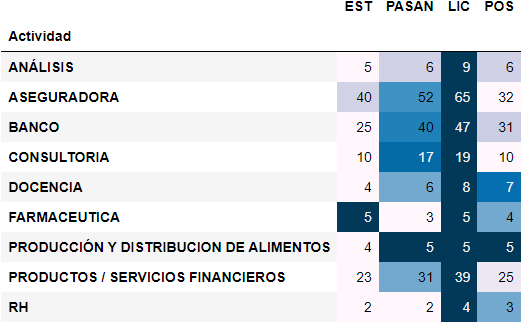
\includegraphics[scale = 0.8]{graf_api_admin.png}
\end{center}

Siendo Licenciado las puertas están prácticamente abiertas para toda Actividad:

\begin{itemize}
    \item Si eres \textbf{Estudiante}, las \textbf{farmacéuticas} considerarán contratarte más que en otros lugares. Las aseguradoras también son una buena opción y en menos proporción, los bancos.
    
    \item Si eres \textbf{Pasante}, empiezas a lucir más atractivo para las empresas y en general no tendrías problema para conseguir un trabajo, particularmente en \textbf{Producción y Distribución de Alimentos}.
    
    \item Con un \textbf{Posgrado}, la actividad de la \textbf{Docencia} añorará tu conocimiento académico. 
\end{itemize}

\subsubsection{Necesito seguir estudiando pero quiero un empleo, ¿en qué Actividad es más probable encontrar un trabajo de jornada parcial?}

\begin{figure}[h!]
\centering
\begin{minipage}{.5\textwidth}
  \centering
  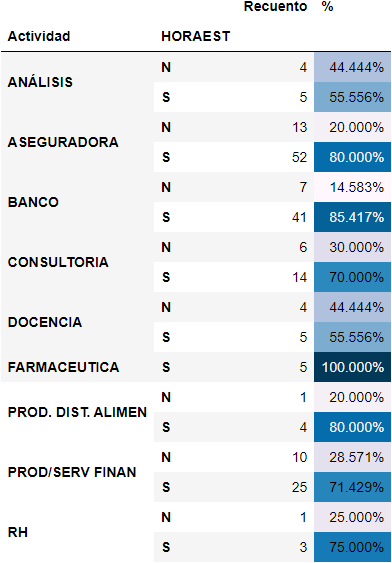
\includegraphics[scale = 0.6]{cru3_api_hora.png}
\end{minipage}%
\begin{minipage}{.5\textwidth}
  \centering
  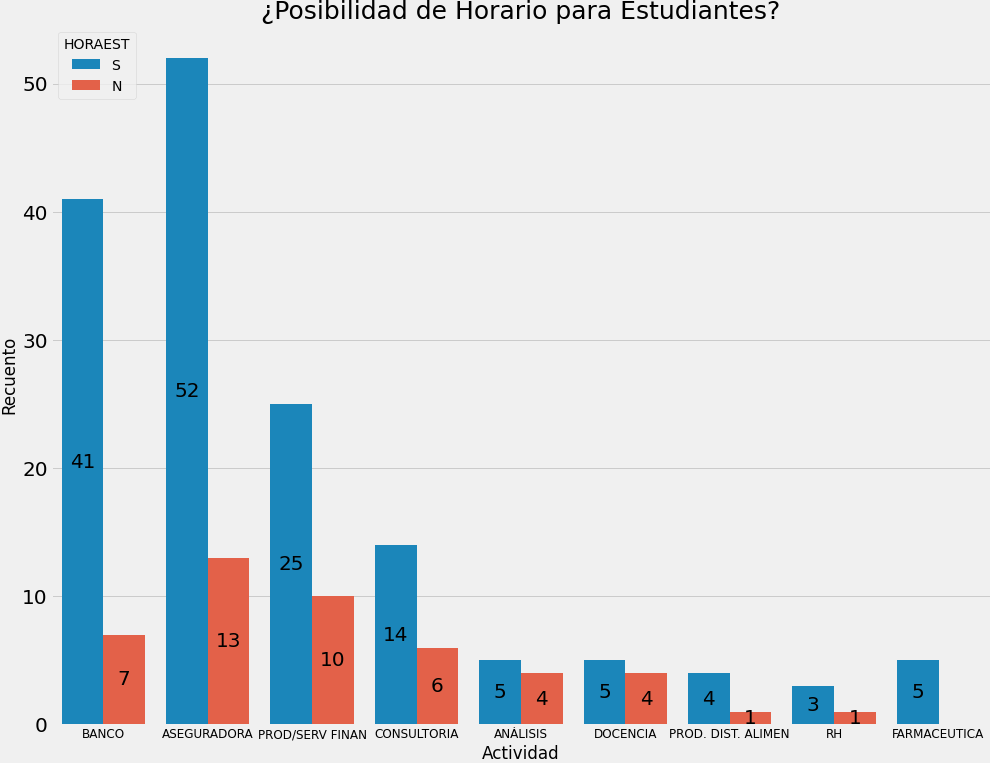
\includegraphics[scale = 0.3]{graf_api_hora.png}
\end{minipage}
\end{figure}
\FloatBarrier

\textbf{Trabajar en una Farmacéutica} puede ser tu opción, pues de todos los registros, absolutamente todos permiten tener un trabajo de medio tiempo. Ahora bien, son \textbf{Análisis y Docencia} las actividades en las cuales puedes tener menos oportunidades, pero ésta afirmación tampoco es tan radical, pues más del $50\%$ de ambas actividades permiten trabajos de medio tiempo. 


\subsubsection{¿Qué promedio mínimo debería tener para ser considerado para una posición dependiendo del área?}

\begin{figure}[h!]
\centering
\begin{minipage}{.5\textwidth}
  \centering
  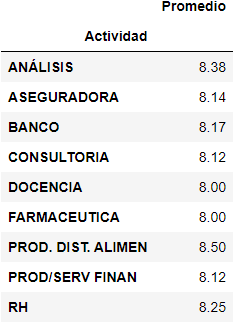
\includegraphics[scale = 0.8]{cru4_api_prom.png}
\end{minipage}%
\begin{minipage}{.5\textwidth}
  \centering
  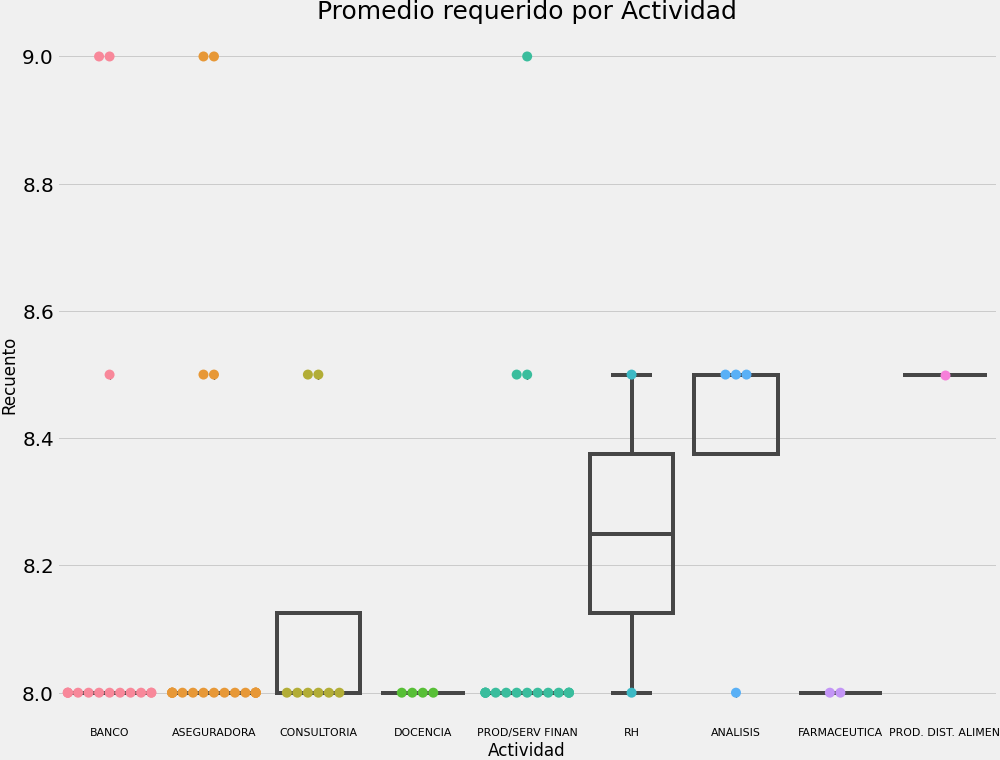
\includegraphics[scale = 0.26]{graf_api_prom.png}
\end{minipage}
\end{figure}

En todos las Actividades es muy posible que te pidan un \textbf{promedio mínimo de 8}.Sin embargo, hay actividades como \textbf{Banco, Aseguradora y Productos y Servicio Financieros} que rara vez pedirán un promedio mínimo de 9. Lo ideal sería tener un promedio \textbf{igual o mayor a 8.5} para poder acceder con mayor seguridad a un puesto en cualquiera de las Actividades de tu interés.

\subsubsection{¿Qué tanto dominio del idioma inglés debo de tener dependiendo de la Actividad para la que aplique?}

\begin{center}
    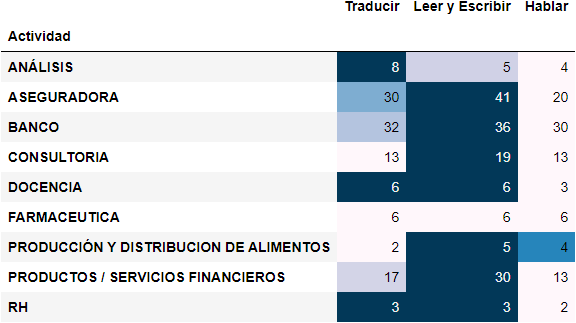
\includegraphics[scale = 0.7]{cru5_api_ingles.png}
\end{center}

Algo es claro: \textbf{Hay que dominar el idioma inglés sí o sí}. Para ciertas actividades se quiere tener dominio particular en ciertas tareas: 

\begin{itemize}
    \item \textbf{Leer y Escribir en inglés} es prioridad para todas las Actividades, con menos fuerza para Análisis.
    
    \item En la \textbf{Docencia} es poco relevante si puedes hablarlo, lo cual tiene sentido al ser más dados a leer documentos y artículos en inglés. 
    
    \item En \textbf{Análisis} se prefiere más la habilidad de \textbf{traducción} que en ningún otra Actividad. 
    
    \item En cuestión de \textbf{aseguradoras: Traducir, Leer y Escribir bien} te dará mucha ventaja competitiva. 
\end{itemize}


\subsubsection{¿Qué tanta experiencia laboral previa necesito para aplicar a mi primer puesto de trabajo dependiendo de la Actividad?}

\begin{center}
    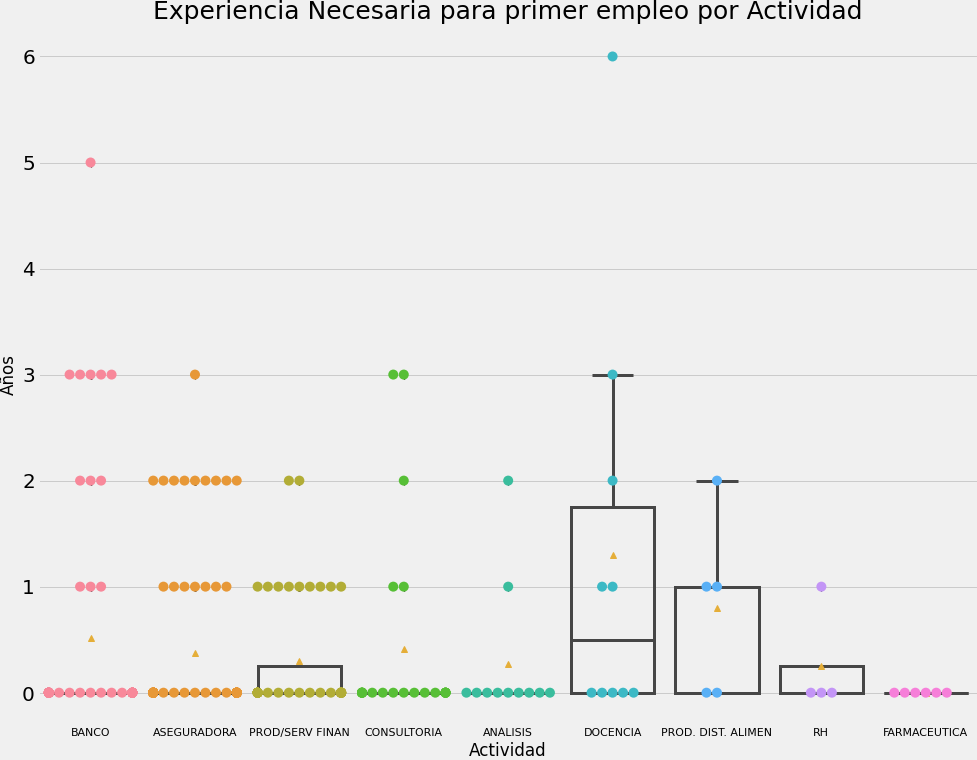
\includegraphics[scale = 0.3]{graf_api_exp.png}
\end{center}

\begin{itemize}
    \item En promedio, se espera que \textbf{todas las Actividades pidan entre 0 y 1.5 años de experiencia}

    \item En particular las \textbf{Farmacéuticas tienden a no requerir de experiencia previa}.
    
    \item Las \textbf{Aseguradoras y los Bancos suelen pedir más años de experiencia}, incluso llegando a los 5 años. 
    
    \item La \textbf{Docencia} es posiblemente la actividad que \textbf{mayor varianza presenta en cuanto a los años requeridos}, así como los valores más atípicos.
\end{itemize}


\subsubsection{¿Existe preferencia por alguna escuela dependiendo de la Actividad?}

\begin{center}
    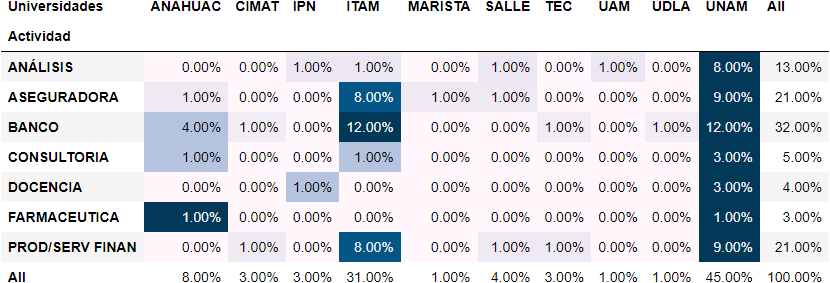
\includegraphics[scale = 0.7]{cruz6_api_pref.png}
\end{center}

\begin{center}
    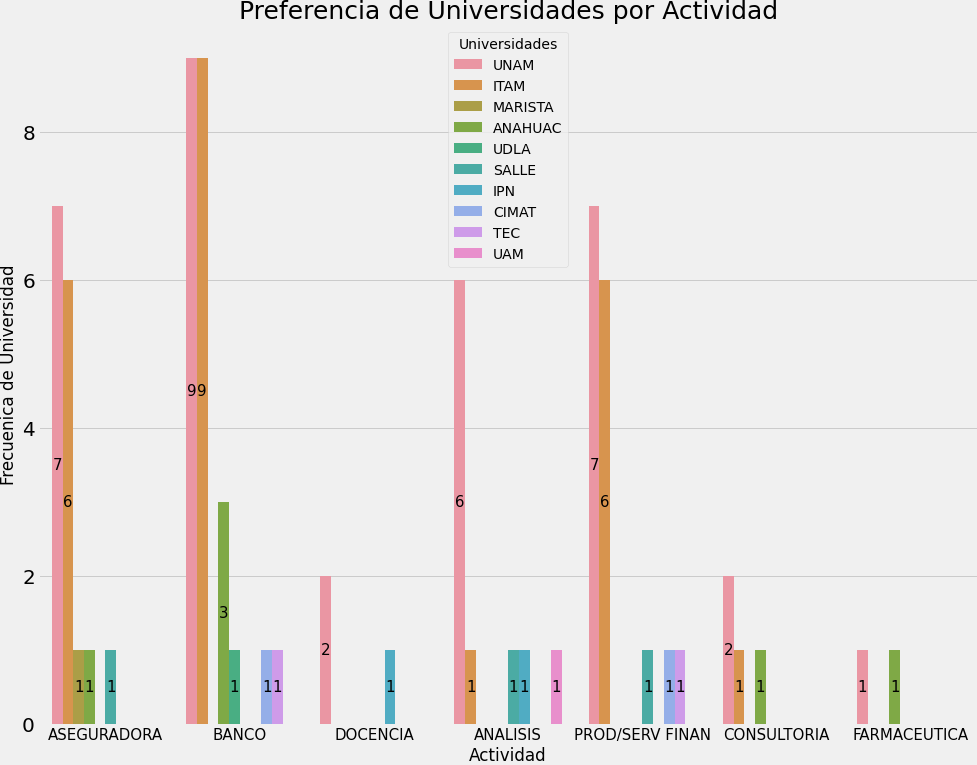
\includegraphics[scale = 0.4]{graf_api_pref.png}
\end{center}

Sí. \textbf{La UNAM y el ITAM} son las escuelas que más preferencia tienen en las Actividades \textbf{Aseguradora, Banco y Productos/Servicios Financieros}, teniendo la UNAM una mayor pero ligera proporción. En temas de \textbf{Análisis, la UNAM domina por completo sobre las demás.} La tercera mejor opción es la Universidad Anahuac, pero no es competencia para las dos primeras mencionadas. La UNAM predomina sobre todas las demás, abarcando casi la mitad de las preferencias totales en todas las Actividades. 




\subsubsection{¿Qué conocimiento técnico me conviene dominar si me gustaría trabajar en una aseguradora, banco o a los servicios financieros?}

\begin{center}
    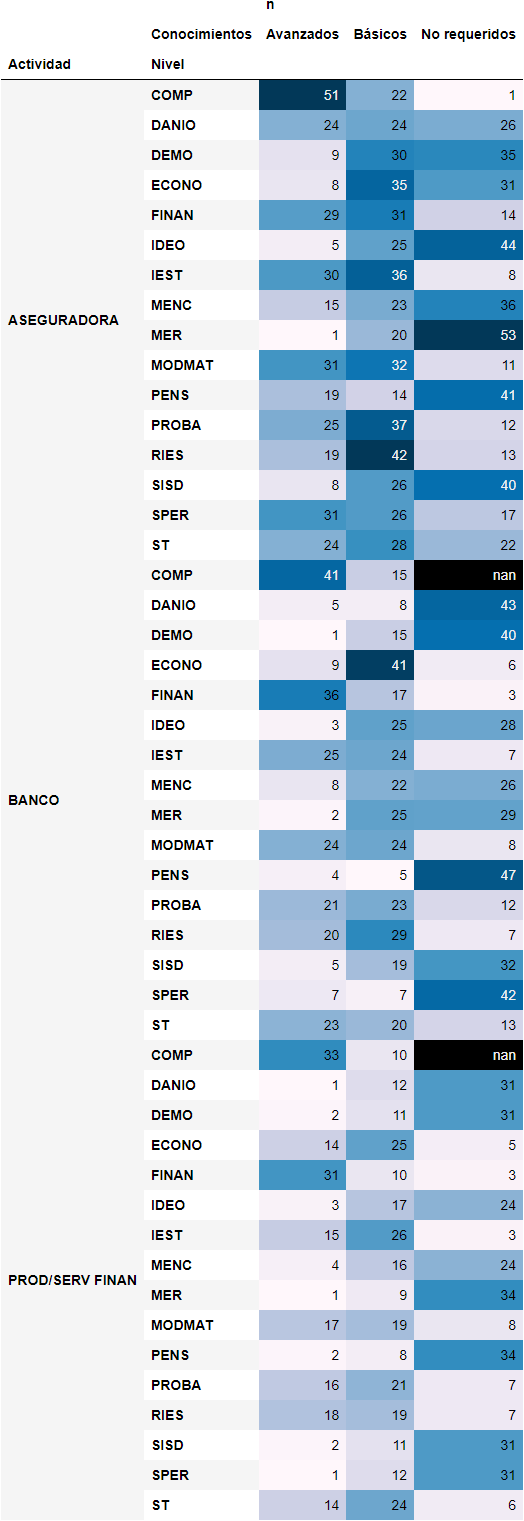
\includegraphics[scale = 0.5]{cruz8_api_materias.png}
\end{center}


\begin{itemize}
    \item \textbf{ASEGURADORAS:} Conocimientos de computación, Inferencia Estadística, Economía y Teoría del Riesgo son vitales para esta actividad. Conocimiento sobre Mercados puede quedar en segundo plano. 
    
    \item \textbf{BANCOS:} Conocimientos sobre Computación y Finanzas son lo más conveniente que domines, así como Economía. Daños, Pensiones y Demografía pueden quedar totalmente fuera de tu arsenal. 
    
    \item \textbf{PROD/SERV FINANCIEROS:} Definitivamente (y trivialmente), Finanzas será tu pan de cada día. Como en todo, la Computación es muy útil, así como tener conocimientos básicos de Economía, Series de Tiempo e Inferencia Estadística. 
\end{itemize}


\subsubsection{¿Qué lenguajes de programación debería manejar dependiendo de la actividad?}

\begin{center}
    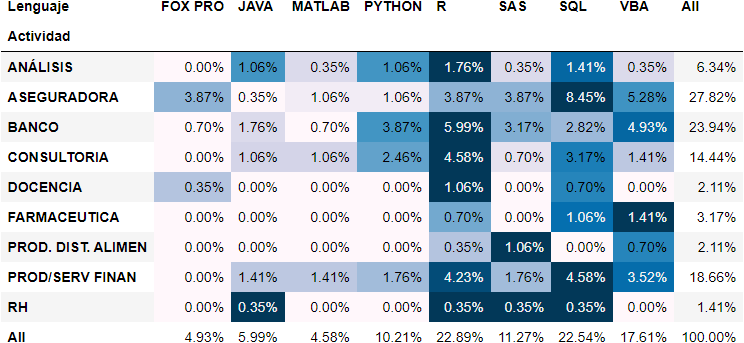
\includegraphics[scale = 0.8]{cru9_api_lenguajes.png}
\end{center}

\begin{center}
    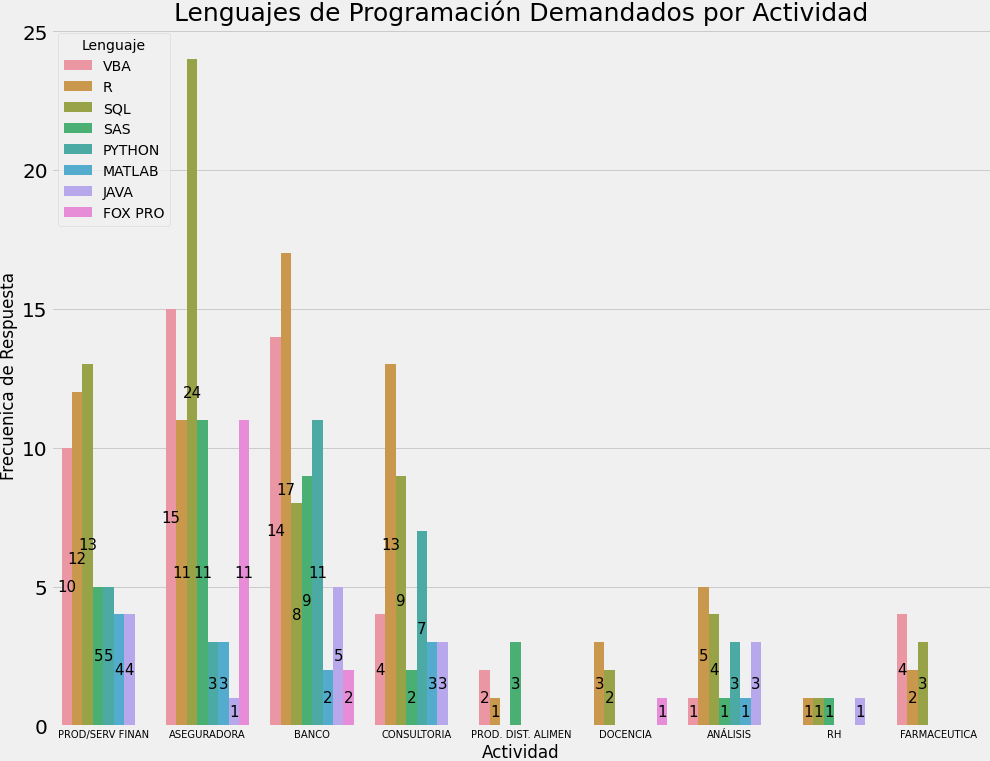
\includegraphics[scale = 0.425]{graf_api_lenguajes.png}
\end{center}


Para el año 2018: 

\begin{enumerate}
    \item Existe una clara demanda del conocimiento del manejo de \textbf{R y SQL} en cualquier Actividad. 
    
    \item En otras áreas más financieras, también se da preferencia a \textbf{SAS}. Indudablemente \textbf{VBA} permanecía como uno de los lideres en esta Actividad.
    
    \item En la actividades como el \textbf{Análisis y Consultoría}, \textbf{Python comienza a agarrar fortaleza}

\end{enumerate}

Para el año 2022, son \textbf{R, pero sobre todo Python,} los lenguajes más solicitados en el mercado laboral. Esto por la creciente necesidad del manejo y modelado de datos, dando paso a la popular Ciencia de Datos. 



\subsubsection{Deficiencias: La opinión de los expertos sobre los fallos más comunes}

\begin{center}
    \includegraphics[scale = 0.35]{graf_deficiencas.png}
\end{center}

En la opinión de todas las personas que ya tienen experiencia sobre lo que es la vida laboral, sin importar a qué se dediquen o dónde trabajen, sobresalen las siguientes carencias que han presentado los nuevos aspirantes:

\begin{enumerate}
    \item Trabajo en Equipo;
    
    \item Falta de Conocimientos Técnicos;
    
    \item Falta de Proactividad;
    
    \item Falta de Experiencia;
    
    \item Falta de Compromiso;
    
    \item Falta de Conocimientos sobre lenguajes de programación y Bases de Datos;
    
    \item Dificultad para la Comunicación Oral;
    
    \item Falta de capacidad para Trabajar bajo presión;
    
    \item Mala ortografía y mala redacción;

\end{enumerate}

Entre otras cosas, se observa que muchas de las deficiencias no corresponden a conocimientos técnicos, sino a habilidades blandas que pocas veces se propicia su desarrollo en la escuela. 

\subsection{Análisis no paramétrico}

\subsubsection{Soy una persona muy creativa y me gustaría trabajar en una aseguradora, banco, consultoría o en servicios/productos financieros, ¿lo anterior me ayudará a conseguir trabajo más fácil en alguna de las Actividades de mi interés?}

Para abordar la siguiente pregunta, optaré por utilizar un enfoque no paramétrico (medidas en escala ordinal) \textbf{Kruskal-Wallis}:

\begin{enumerate}
    
    \item \textbf{Cantidad de datos por grupo}: aseguradora (74), banco (56), servicios/productos financieros (44) y consultoría (24). 
    
    \item \textbf{Normalidad en los datos por grupo:} Definitivamente no se cumplirá la normalidad en los datos. Esto lo confirma el \textit{Test de Jarque-Bera} aplicado a cada uno de los 4 grupos analizados. Tanto el grupo de Aseguradora como Banco y servicios/productos financieros  (mayores datos), la hipótesis nula de normalidad fue rechazada con P < .001; por otra parte, bajo un nivel de riesgo de 0.05, el conjunto de datos de Consultoría no rechaza la hipótesis nula de normalidad con P = .07. Así, se concluye que no puede ser utilizado (o no es aconsejable) un método paramétrico como ANOVA de una vía. 
    
    \item \textbf{Varianza}: Bajo el \textit{Test de Levene}, no se rechaza la hipótesis nula de homogeneidad con P = .52. Esto es claro, porque los valores solo varían entre 1 y 5 en todas los conjuntos de datos.
    
    \item \textbf{Similitud entre distribuciones}: Se observa una distribución bastante similar para todas las Actividades, una condición esencial para el uso de Kruskal-Wallis. 
\end{enumerate}

\begin{center}
    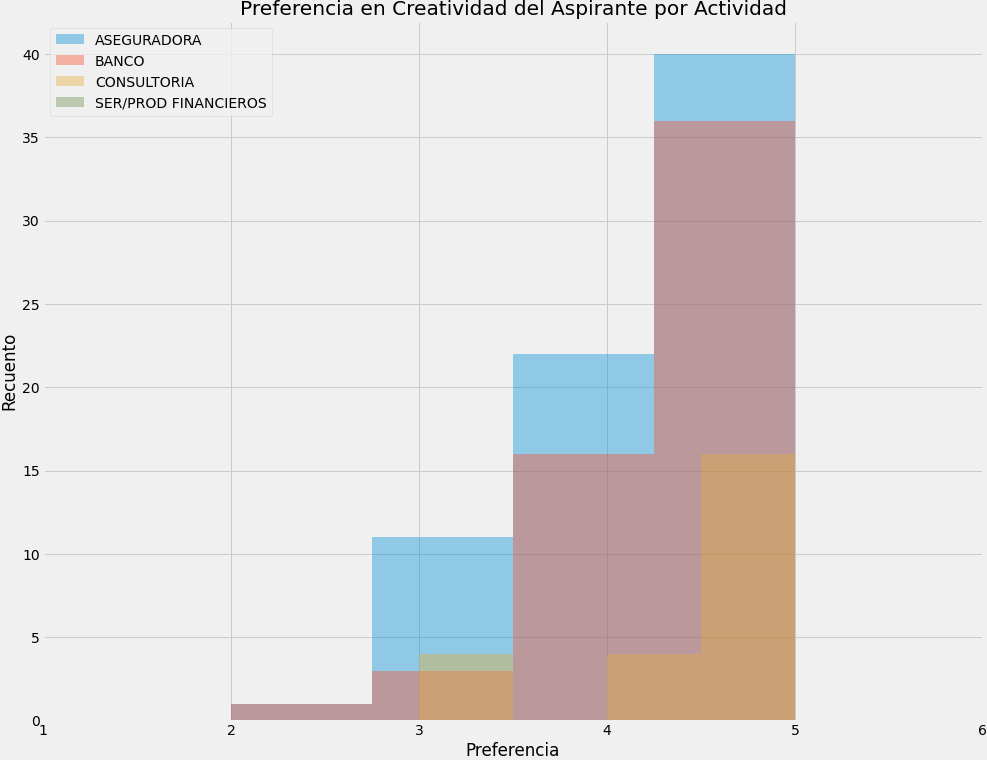
\includegraphics[scale = 0.3]{graf_CREA.png}
\end{center}


Después de probar que se cumplen con todas los supuestos, se realiza el test, obteniendo un \textbf{P = .48}, evidencia suficiente para no rechazar la hipótesis nula de la diferencia de medias. Esto es, no existe una diferencia entre la demanda de creatividad entre todas las Actividades que te gustan, TODAS te lo van a requerir. Este no será un diferenciador a la hora de aplicar para un puesto.  


\begin{center}
    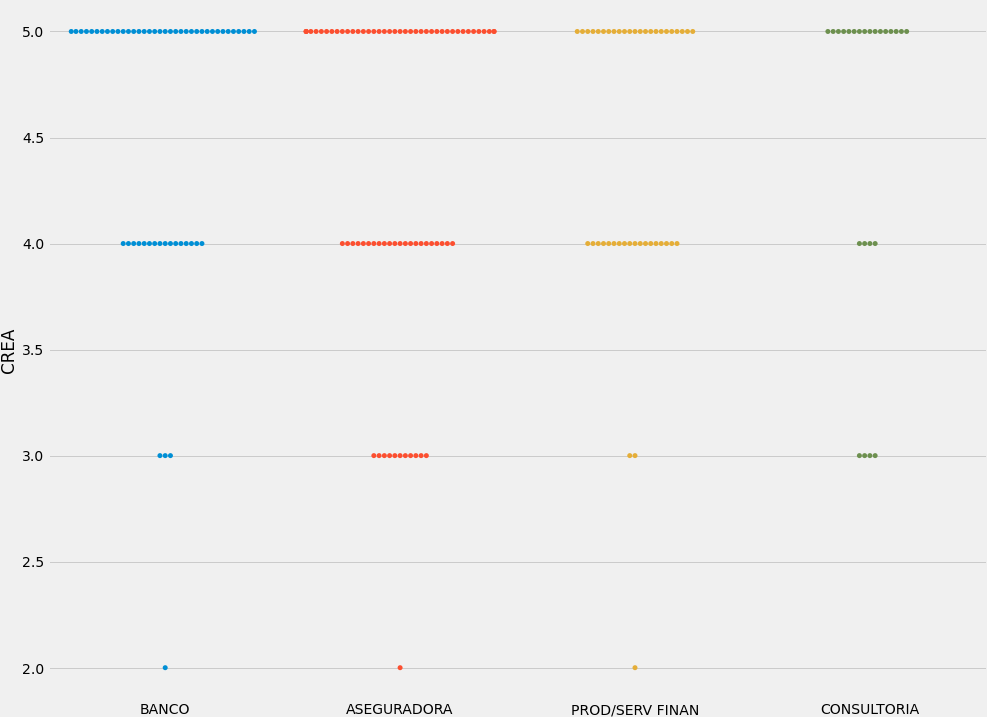
\includegraphics[scale = 0.3]{graf_CREA2.png}
\end{center}

Aún cuando se han dado las razones por las cuales no se debería de efectuar un análisis ANOVA, por curiosidad, se obtuvo un \textbf{P = .52}, conclusión muy similar a la propuesta por Kruskal-Wallis. 


\subsubsection{Por qué no es buena idea aplicar métodos paramétricos a estos datos}

La distribución de los datos contenidos en el conjunto de datos son, en su mayoría, ordinales. Si bien, se pueden utilizar bajo ciertos argumentos algunos métodos no paramétricos para analizar este tipo de datos, no es lo recomendable. Además, los datos en general no presentan mucha variabilidad e intuitivamente se conoce la distribución de los datos por cada atributo. Es así como se llega a la conclusión de que en este tipo de datos en la que la incertidumbre concerniente a la distribución de los datos es prácticamente inferida de manera empírica, no vale la pena aplicar este tipo de análisis. 




\section{CONCLUSIONES}

La actuaría fue, sigue siendo y seguirá siendo una de las carreras más prometedoras y con mayor cantidad de salidas laborales una vez terminados los estudios universitarios. Si bien la carrera es relativamente nueva y aún hay mucho por mejorar en los planes de estudio de las universidades mexicanas, es cierto que como estudiante uno debe de añorar la mejora continua y ser autodidactas y autosuficientes al momento de adquirir nuevas habilidades que pocas veces se ponen en práctica en la escuela como lo son las habilidades blandas y sociales. En el presente trabajo se ilustró cuáles eran las necesidades y conocimientos que los estudiantes recién egresados de la carrera deberían tener a la hora de aspirar por una oportunidad laboral. Así mismo, se llegó a la conclusión de que dependiendo de la Actividad que realice cierta empresa estos requerimientos podrían cambiar. Un punto muy importante a enfatizar es que, como actuarios, debemos ser más empáticos y entender que trabajaremos rodeados de gente que no conoce nuestro idioma matemático. Debemos de tener en mente que muchas veces es más importante explicar a un contador lo que hacemos en términos sencillos que saber realizar una integral a mano. \\

Con el paso del tiempo el conocimiento de matemáticas será algo que todo mundo deberá dominar para poder adaptarse a las necesidades que el propio futuro nos depara. El actuario es capaz de encontrar respuestas a problemas complejos, así como de ahogarse en un vaso de agua si no sabe explicar la solución a aquellos problemas. 


\section{RECOMENDACIONES}

A lo largo del procesamiento y limpieza de los datos, me percaté de que los datos tenían muchos \textbf{errores en cuanto a la captura de los datos}. Esto dificultó mucho el análisis descriptivo; tardaba más tiempo tratando de agrupar y unificar las categorías textuales recabadas que formulando la pregunta que iba a responder. Es bien sabido que estos son problemas que día a día se presentan en documentos del calibre INEGI, pero, ciertamente, en nuestro caso pudieron ser corregidos sí desde el inicio hubiéramos restringido las entradas en el \textit{Google Forms} dependiendo de la pregunta; es decir, en lugar de hacer los campos libres, mejor utilizar preguntas de opción múltiple o listas desplegables. Si el encuestado no se decidía por alguna de esas opciones, habilitar una respuesta como 'otra' y permitir ahora sí escribir su respuesta personal. \\

Otro problema al que me enfrente fue la \textbf{falta de datos} que, en mi opinión, no transgredían la intimidad del encuestado: Sexo, Licenciatura Estudiada y dónde la estudio, Años de Experiencia en el Ramo actual, etc. Esto crea nuevos puntos de vista de análisis para evitar sesgos. Por ejemplo, dado que somos estudiantes de la UNAM, tendremos más contacto con gente de la UNAM y esto se ve reflejado en el apartado de \textbf{Preferencias}. \\

Además, propondría \textbf{plantear preguntas sobre temas que de verdad desconozcamos}. Por ejemplo, es muy bien sabido que todos los contratantes buscarán en un aspirante que sea creativo, bueno para hablar en público y bueno para explicar sus ideas de la mejor forma; esto lo confirma el sesgo tan evidente que presentan este tipo de preguntas hacia los valores 3, 4 y 5 en escala likert. \\

Del 2018 al 2022 ya se han modificado radicalmente las habilidades, aptitudes y formas de trabajar, considerando lo introducido por la necesidad de adaptación ante la pandemia. Muchas cosas como 'Contratación por periódico' son, actualmente, obsoletas. Una pregunta nueva (por dar un ejemplo) sería: ¿Qué esquemas de trabajo maneja tu empresa: Híbrido, Online o Presencial?


\end{document}
